\documentclass[12pt]{article}
\RequirePackage{amsthm,amsmath,amsbsy,amsfonts}
\usepackage{graphicx}
%\usepackage{enumerate}
\usepackage{natbib}
\usepackage{url} % not crucial - just used below for the URL 
\usepackage{placeins}

%\pdfminorversion=4
% NOTE: To produce blinded version, replace "0" with "1" below.
\newcommand{\blind}{0}

% DON'T change margins - should be 1 inch all around.
\addtolength{\oddsidemargin}{-.5in}%
\addtolength{\evensidemargin}{-.5in}%
\addtolength{\textwidth}{1in}%
\addtolength{\textheight}{1.3in}%
\addtolength{\topmargin}{-.8in}%


\begin{document}
	\title{Supplementary Material}	 
	
	\section{ADMM details}
	We first re-parameterize $\phi_j = y-\theta_j$ so the problem is
	\begin{equation}
	\text{minimize } \rho_\tau(\phi) + \lambda||D^{(k)}(y-\phi)||_1\\
	\end{equation}
	
	
	We further divide $\phi$ order to solve smaller problems: Defining
	\begin{align}
	&\phi_1 = (\phi_{11}, \phi_{12})\\
	&\phi_2 = (\phi_{21}, \phi_{22}, \phi_{23})\\
	&\phi_3 = (\phi_{31}, \phi_{32})\\
	&\phi = (\phi_{11}, \phi_{12}=\phi_{21}, \phi_{22}, \phi_{23}=\phi_{31}, \phi_{32}) \\
	\end{align}
	Dividing $y$ similarly, the problem then becomes 
	\begin{align}
	&\text{minimize } \sum_{i=1}^3 \rho_\tau(\phi_i) + \lambda||D^{(k)}(y_i-\phi_i)||_1\\
	&\text{subject to: } \phi_{12}=\phi_{21}, ~~ \phi_{23}=\phi_{31}\\
	\end{align}
	We can further simplify by defining 
	\begin{align}
	&\overline{\phi} = (\phi_{11}, \frac{\phi_{12}+\phi_{21}}{2}, \phi_{22}, \frac{\phi_{23}+\phi_{31}}{2}, \phi_{32}) \\
	&\overline{\phi_1} = (\phi_{11}, \frac{\phi_{12}+\phi_{21}}{2})\\
	&\overline{\phi_2} = ( \frac{\phi_{12}+\phi_{21}}{2}, \phi_{22}, \frac{\phi_{23}+\phi_{31}}{2})\\
	&\overline{\phi_3} = (\frac{\phi_{23}+\phi_{31}}{2}, \phi_{32})
	\end{align}
	so the problem becomes
	\begin{align}
	&\text{minimize } \sum_{i=1}^3 \rho_\tau(\phi_i) + \lambda||D^{(k)}(y_i-\phi_i)||_1\\
	&\text{subject to: } \phi_{i}=\overline{\phi_i}\\
	\end{align}
	The augmented Lagrangian for this problem is 
	\begin{align}
	&L_\gamma(\phi_1,\phi_2, \phi_3, \overline{\phi_1}, \overline{\phi_2}, \overline{\phi_3}, \omega) = \\
	&\sum_{i=1}^3 \rho_\tau(\phi_i) + \lambda||D^{(k)}(y_i-\phi_i)||_1 + \omega_i^T(\phi_i - \overline{\phi_i}) + \frac{\gamma}{2}||\phi_i - \overline{\phi_i}||_2^2
	\end{align}
	The ADMM updates are then given by
	\begin{align}
	&\phi_i^{k+1} = \arg\min_{\phi_i}\rho_\tau(\phi_i) + \lambda||D^{(k)}(y_i-\phi_i)||_1 + \omega_i^{kT}(\phi_i - \overline{\phi_i}^k) + \frac{\gamma}{2}||\phi_i - \overline{\phi_i}^k||_2^2\\
	&\omega_i^{k+1} = \omega_i^{k} + \gamma(\phi_i^{k+1} - \overline{\phi_i}^{k+1})
	\end{align}
	The $\phi_i$ updates can be obtained using a quadratic program solver such as Gurobi and can be obtained in parallel. 
	
	\section{Simulation Metrics}
	
	\begin{figure}[h!]
		\caption{F1 score by threshold, data size, and method (1 is best 0 is worst).}
		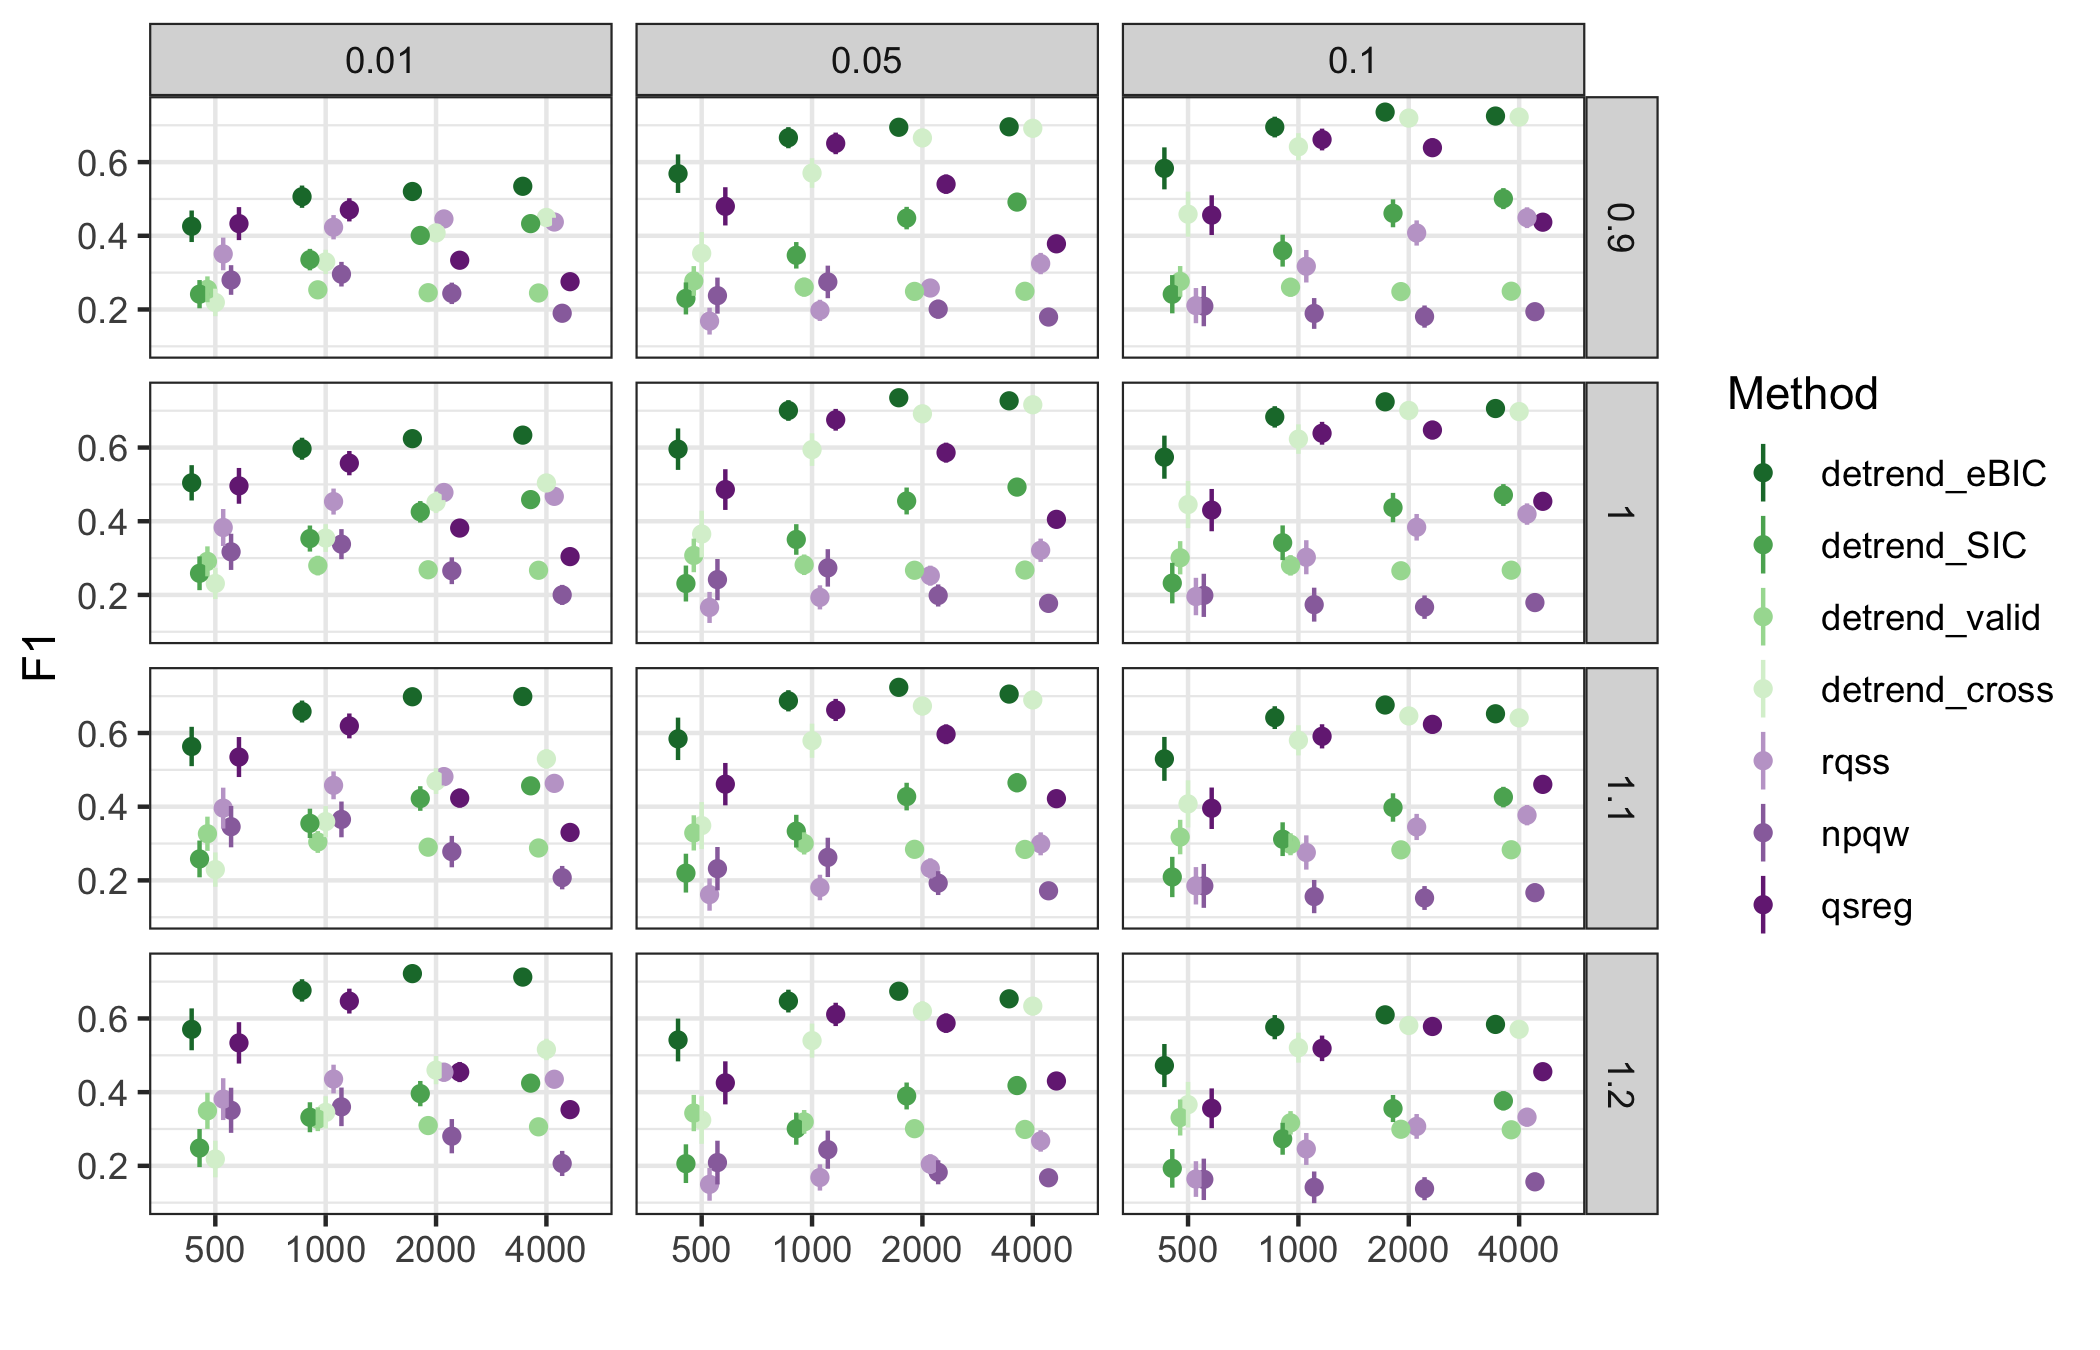
\includegraphics[width = \linewidth]{Figures/peaks_F1.png}
	\end{figure}
	
	\begin{figure}[h!]
		\caption{Precision by threshold, data size, and method (true positive over true positives + false positives).}
		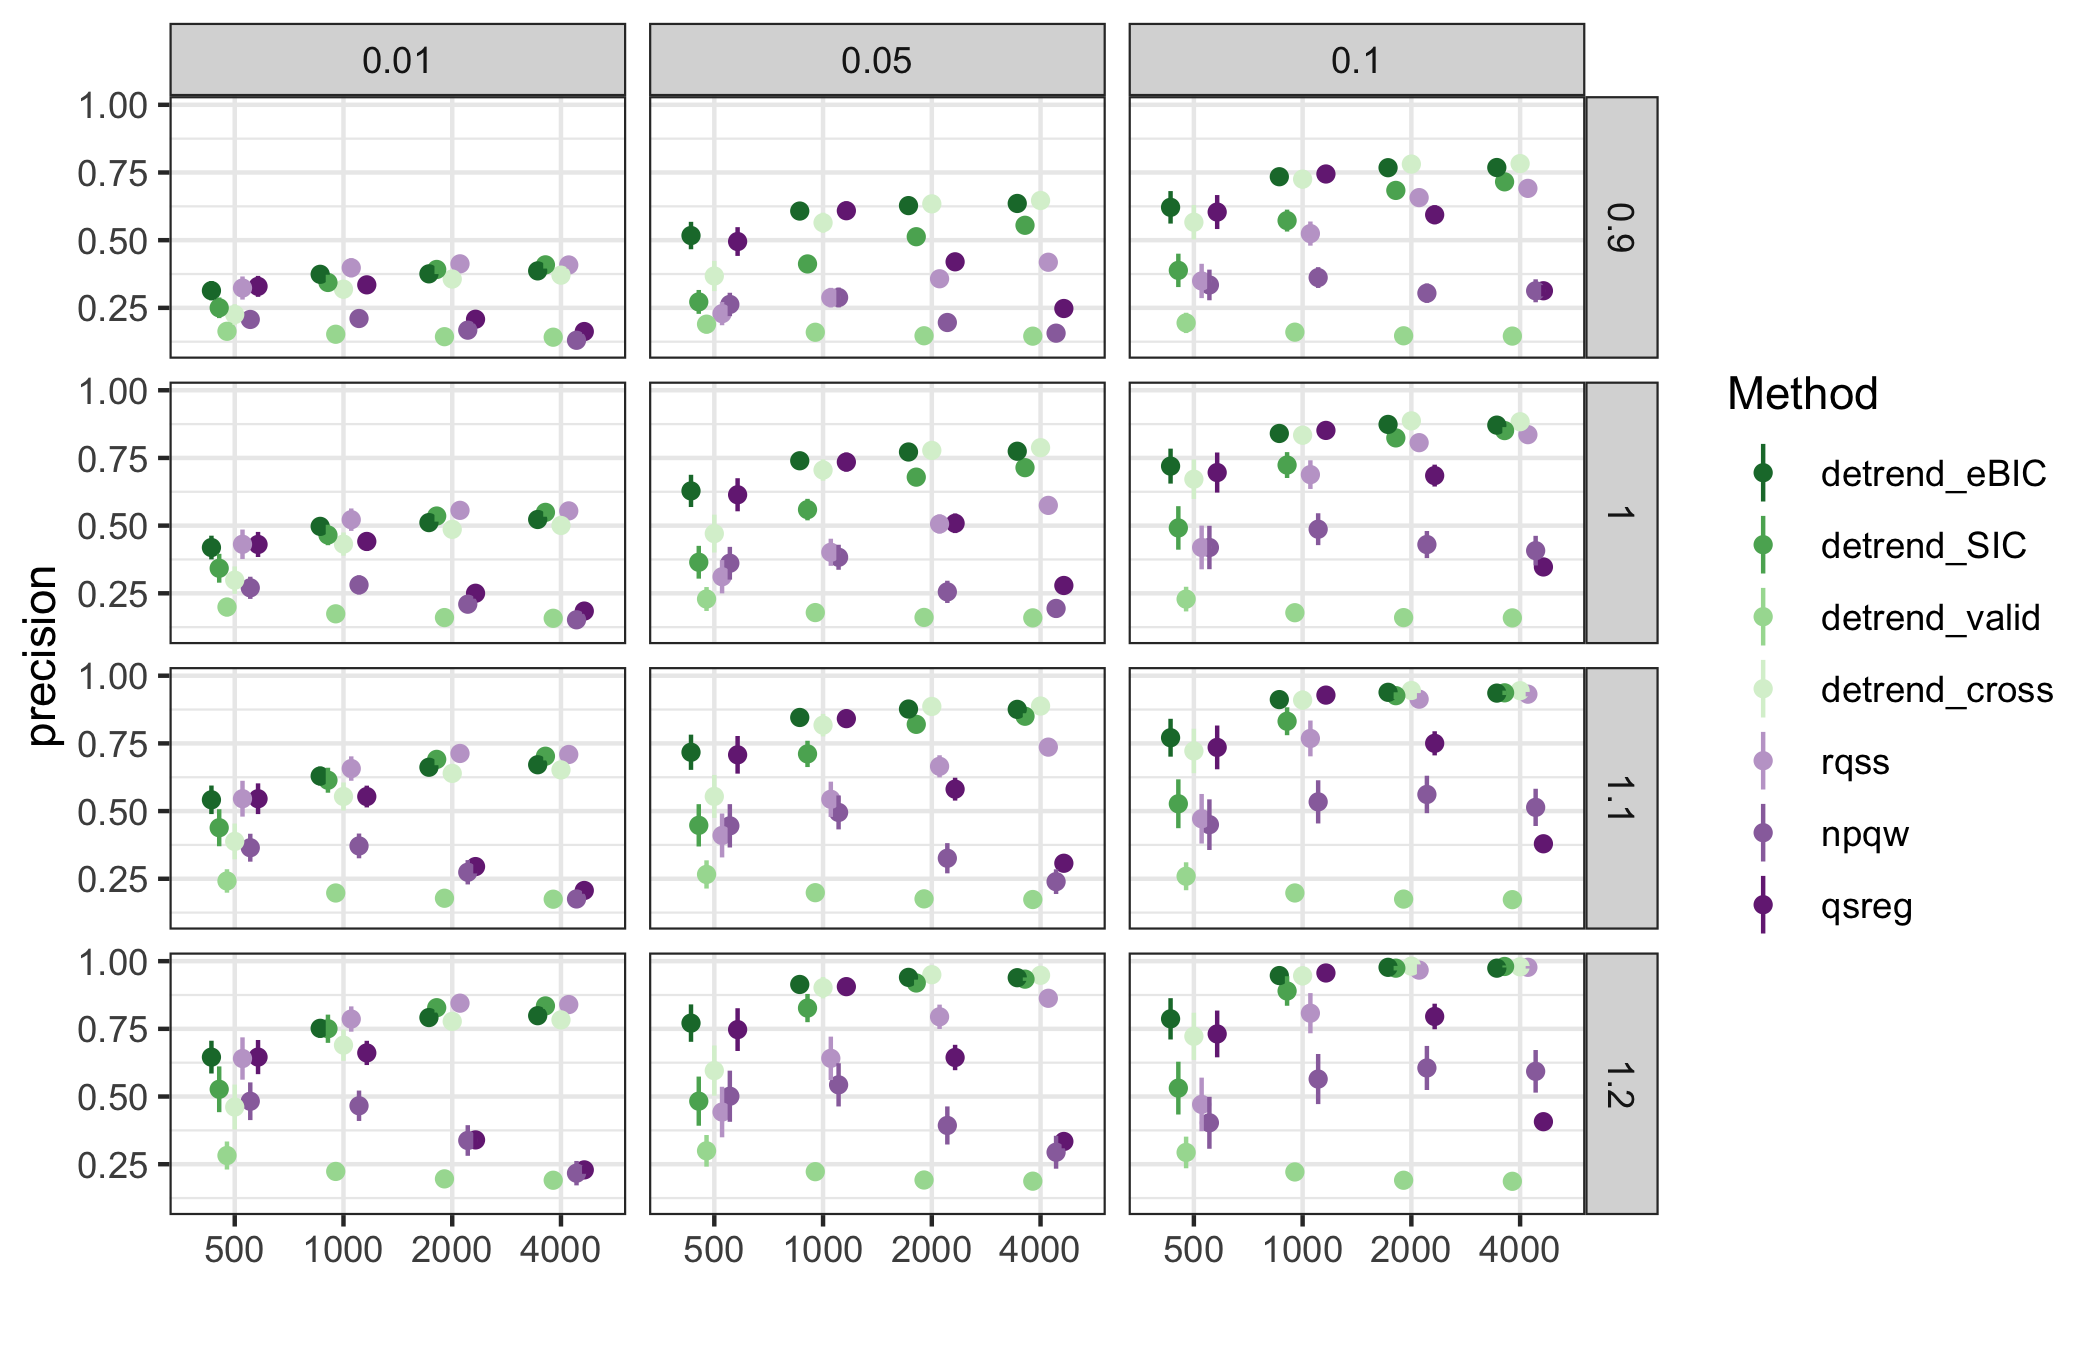
\includegraphics[width = \linewidth]{Figures/peaks_precision.png}
	\end{figure}
	
	\begin{figure}[h!]
		\caption{Recall by threshold, data size, and method (true positive over true positives + false negatives).}
		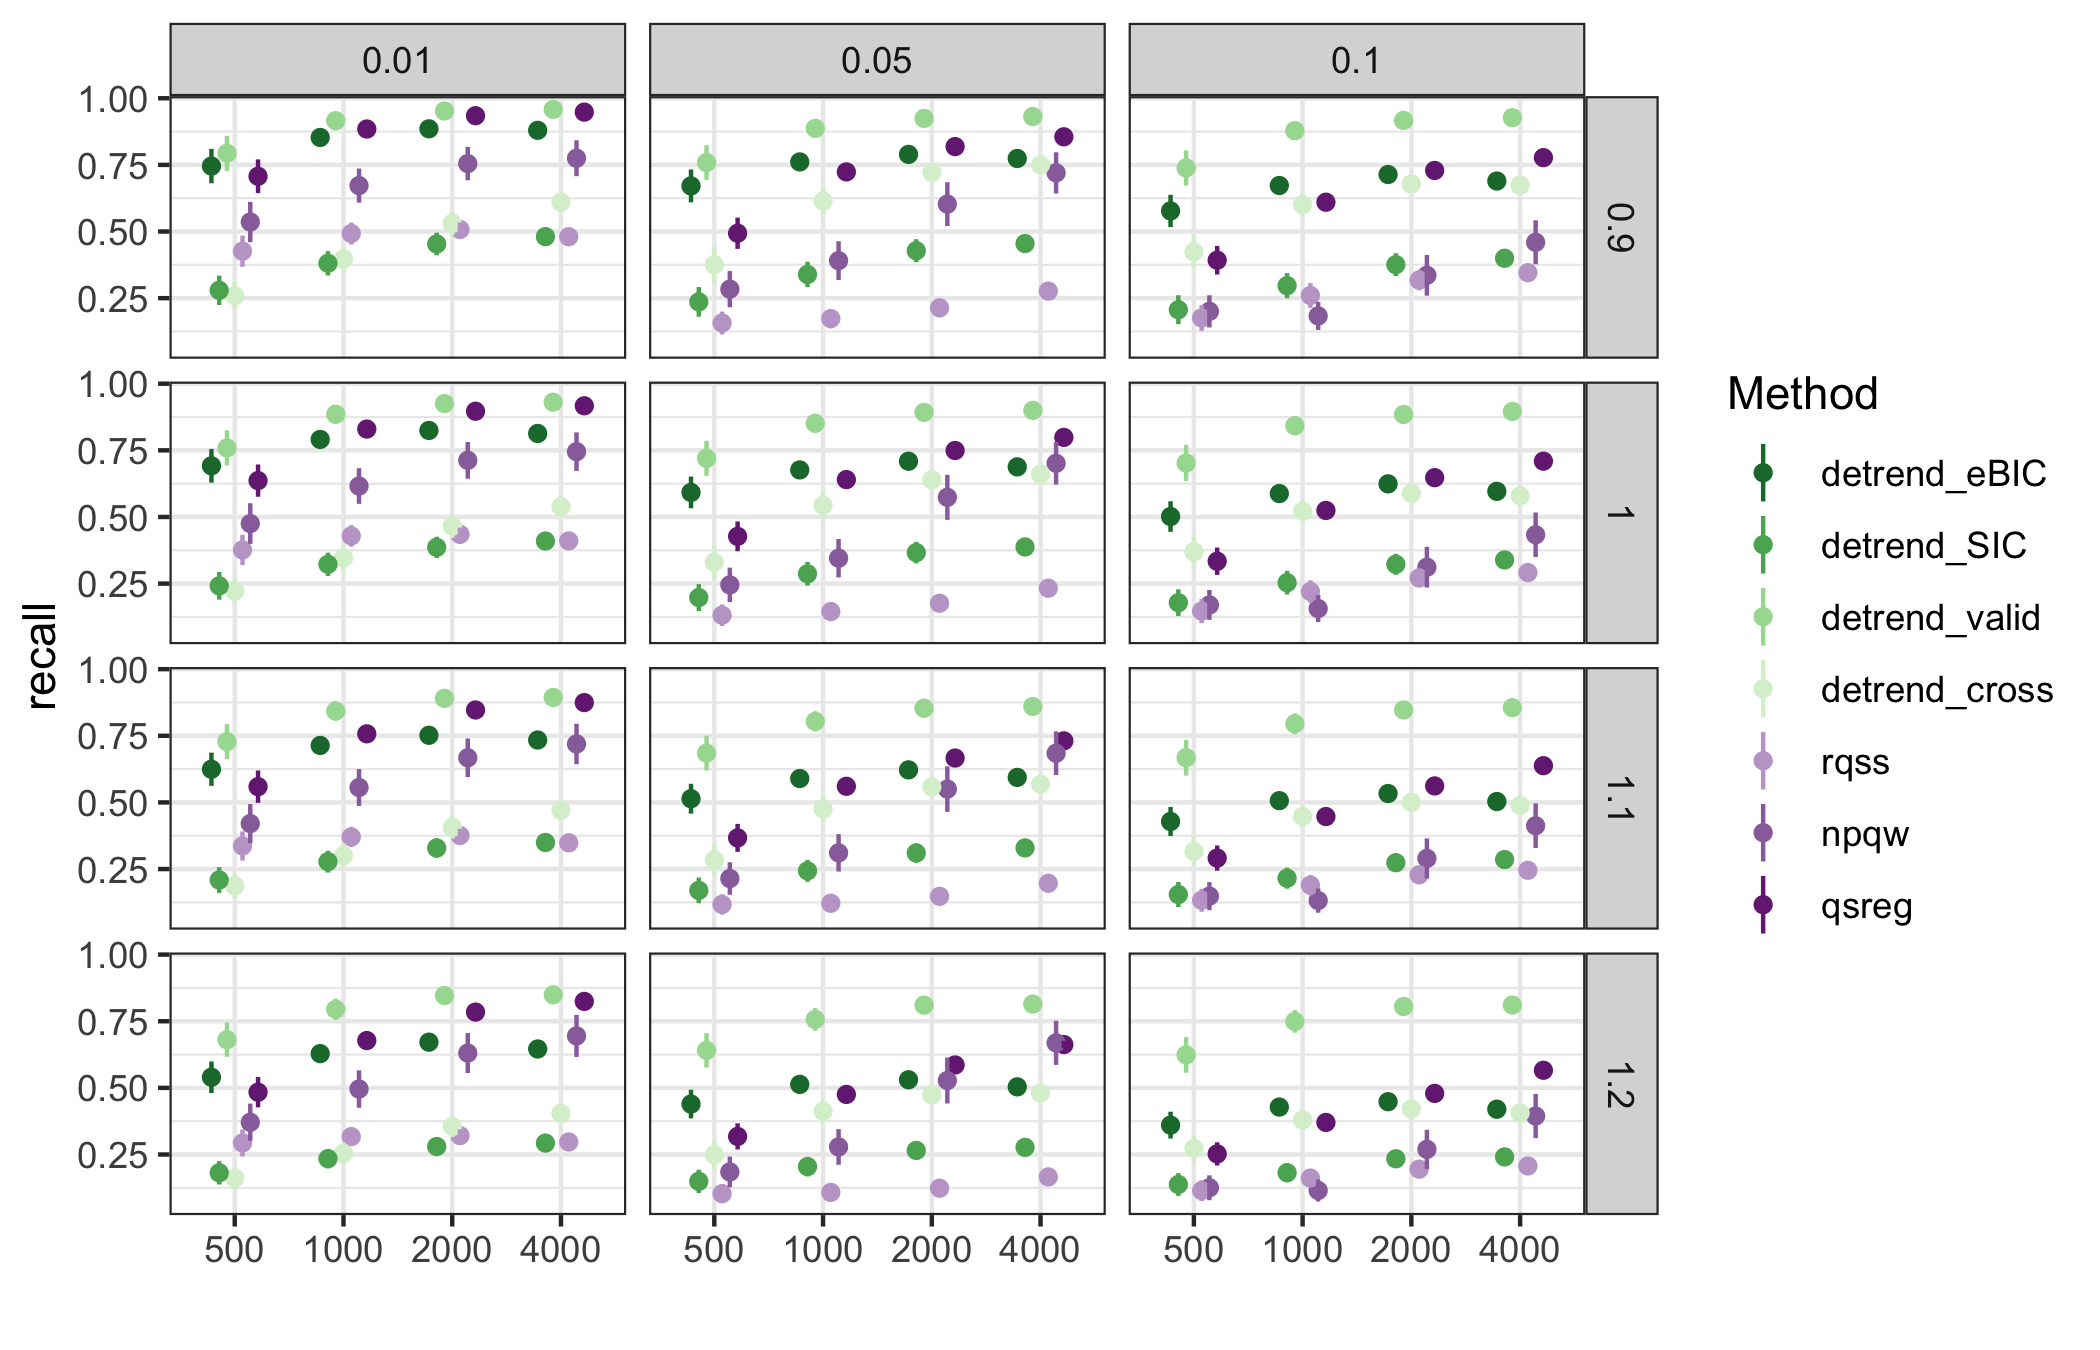
\includegraphics[width = \linewidth]{Figures/peaks_recall.png}
	\end{figure}
	
	\begin{figure}[h!]
		\caption{Miss-classification rates by threshold, data size, and method, values above the upper limit (npqw) not shown.}
		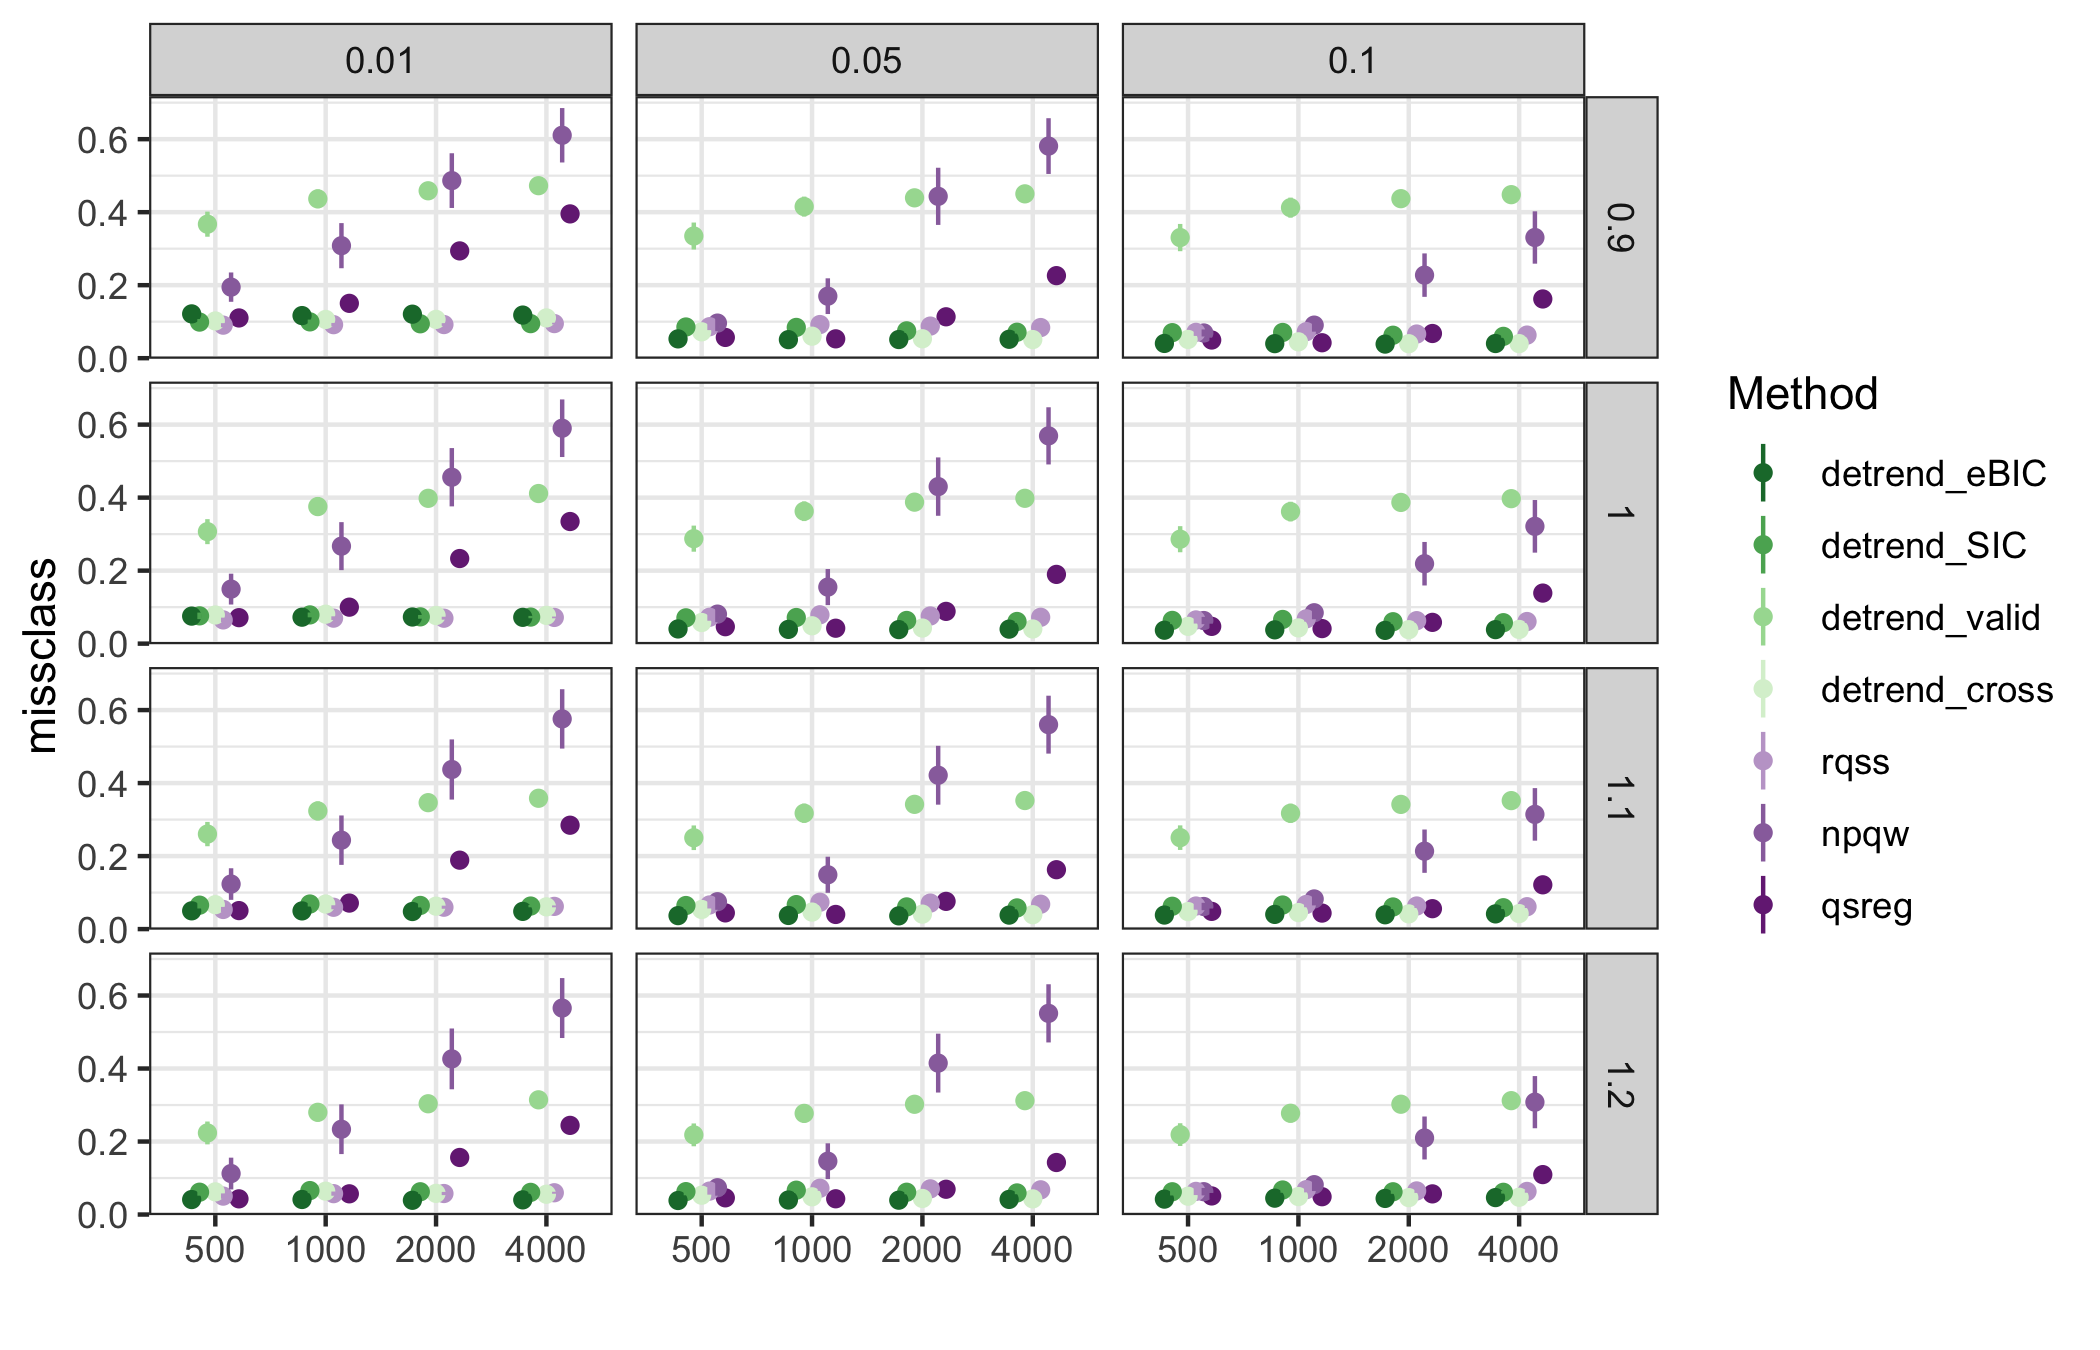
\includegraphics[width = \linewidth]{Figures/peaks_missclass.png}
	\end{figure}

\end{document}